\documentclass[12pt,journal,compsoc]{IEEEtran}

% *** MATH PACKAGES ***
%
\usepackage[cmex10]{amsmath}
\usepackage{amssymb}
% \usepackage{algpseudocode}
\usepackage{graphicx}
\graphicspath{{./images/}}
\DeclareGraphicsExtensions{.jpg,.png}
\usepackage{listings}
\lstset{
basicstyle=\small\ttfamily,
columns=flexible,
breaklines=true
}

\begin{document}
%
% paper title
% can use linebreaks \\ within to get better formatting as desired
% Do not put math or special symbols in the title.
\title{IAML - Assignment 2}
\author{s1474146}

% The paper headers
\markboth{IAML - Assignment 2 - Due Oct 30, 2014}%
\maketitle

%------------------------------------
% Exploration of the dataset
%------------------------------------

\section{Exploration of the dataset}

%------------------------------------
% 1.a
%------------------------------------
\subsection*{1.a}
Accuracy of classifier:
\begin{itemize}
\item SimpleLogistic: 64%
\item Logistic: 66.8%
\end{itemize}

The difference between \texttt{SimpleLogistic} and \texttt{Logistic} are \textbf{XXX}

Using \texttt{InfoGainAttributeEval}, \textbf{XXX - fill in the result}. The reason for different performance in those 2 classifiers are \textbf{XXX}


%------------------------------------
% 1.b
%------------------------------------
\subsection*{1.b}
The role \texttt{ridge} parameter are \textbf{XXX}

Compare regularization to feature selection \textbf{XXX}

Interpret the result \textbf{XXX}

A graph can be seen in Fig. \ref{ridge_chart}. \textit{X-axis} is drawn in log-scale in order that any trend is fully visible.

\begin{figure}
\label{ridge_chart}
\caption{Ridge \& Percent of correct with Logistic Regression}
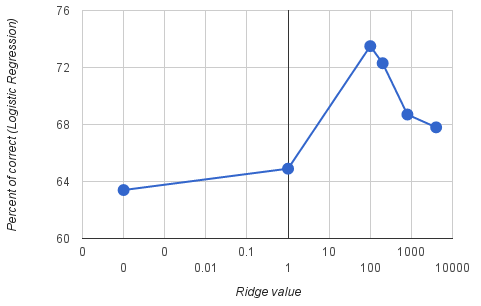
\includegraphics[scale=0.6]{ridge_accuracy}
\end{figure}

%------------------------------------
% 1.c
%------------------------------------
\subsection*{1.c}
\textbf{XXX Explore} the effect of \texttt{gamma}. See Fig. \ref{gamma_chart}

\begin{figure}
\label{gamma_chart}
\caption{Gamma \& Percent of correct with SVM Classifier}
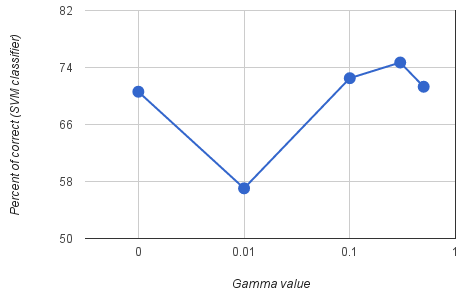
\includegraphics[scale=0.6]{gamma_accuracy}
\end{figure}

\textbf{XXX Explore} the effect of \texttt{complexity parameter}. See Fig. \ref{complexity_chart}

\subsection*{1.c}
\begin{figure}
\label{complexity_chart}
\caption{Gamma \& Percent of correct with SVM Classifier}
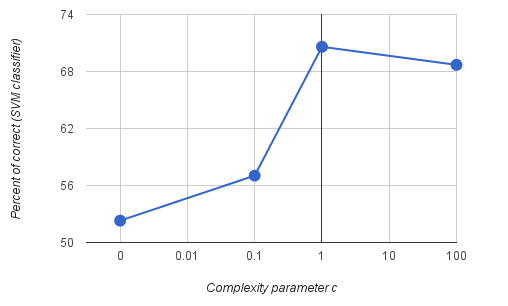
\includegraphics[scale=0.6]{complexity_accuracy}
\end{figure}

This procedure does not guarantee to find the values of \texttt{gamma} and \texttt{c} that lead to the highest percentage correct (PC). Since \textbf{XXX}

%------------------------------------
% 1.d
%------------------------------------
\subsection*{1.d}
Look at the list of the best 50 features, there are 3 \textit{class indicator} variables in that list. The class indicator variable \texttt{is\_bird} is ranked quite high in the list, at position 5. \texttt{is\_cat} and \texttt{is\_aeroplane} follows with position 18, and 22 respectively. \textbf{OOO}

The \texttt{SimpleLogistic} was trained on \texttt{train\_images\_partA}, there are 2 versions: (i) dataset with \texttt{imaId} removed, (ii) dataset with \texttt{imgId} and all the class indicator variables (except \texttt{is\_person}) are removed. Then the classifier are tested on the validation set with the appropriate attributes removed. PC result:

\begin{itemize}
\item Remove \texttt{imgId}, keep all \textit{class indicator variables}: 76.46%
\item Remove \texttt{imgId}, remove all \textit{class indicator variables} but \texttt{is\_person}: 69%
\end{itemize}

\textbf{XXX Relate} the result to the observed feature ranking.

It \textbf{would/would not XXX} be easy to make use of the results in practice. And the reasons are \textbf{XXX}

%------------------------------------
% Mini Challenge
%------------------------------------
\section{Mini Challenge}
\subsection*{Dataset exploration}
Validation set

\begin{itemize}
\item Look at validation set, the only class indicator variable is \texttt{is\_person}.

\item Looking at the histogram of 500 dimensions, this shape of distribution can be seen accross the majority of dimension. Most of the data is concentrated on the left-side, and the tail gets thinner toward the right side.

\item For the majority of dimension, the value lies within range [0, 0.02]

Training set
\item For the majority of dimension, the value lies within range [0, 10]. And the distribution is heavily skewed toward the left side. There are only 1\% of the instance (around 20 instances) that have 
\includegraphics[scale=•]{•}
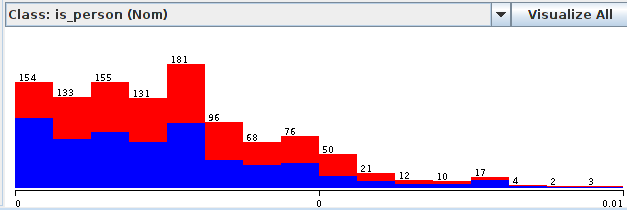
\includegraphics[scale=0.3]{264_val}
\end{itemize}



Preprocessing data for training set

% that's all folks
\end{document}


